\section{Background}
\label{sec:background}

\subsection{Transformer Models}
\label{subsec:transformer_models}
Transformer architectures have emerged as a dominant paradigm in
natural language processing. Unlike traditional recurrent neural
networks and convolutional neural networks, transformers avoid
sequential processing in favour of self-attention mechanisms that
allow for parallel processing of input sequences.

The key innovation of transformers lies in their ability to capture
long-range dependencies within input sequences, making them
particularly effective for tasks such as language translation, text
generation, and sentiment analysis. Models such as \gls{BERT} and
\gls{GPT} have achieved state-of-the-art performance on various
natural language processing benchmarks,
demonstrating the power of transformer architectures.

\subsection{Quantum-Inspired Machine Learning}
\label{subsec:quantum_inspired_machine_learning}

\gls{QiML} refers to a class of machine learning algorithms that draw
inspiration from quantum mechanics but are implemented on classical
hardware. Unlike \gls{QML}, which relies on quantum computation to
process data, \gls{QiML} applies quantum principles to classical
algorithms without the need for quantum devices. \gls{QiML} has
gained attention due to its potential to harness computational
advantages by simulating quantum effects through classical
frameworks. Techniques such as tensor networks, dequantized
algorithms, and quantum-inspired optimisation algorithms are
prominent examples of \gls{QiML} approaches. These methods have been
shown to improve efficiency and performance on certain tasks
traditionally solved using classical machine learning models.

The relationship between \gls{QiML} and \gls{QML} can be understood
as a spectrum of quantum mechanics integration, as illustrated in
Figure~\ref{fig:qiml_levels}. On the left side of the spectrum, we
have classical approaches
like dequantized algorithms that employ quantum-inspired techniques
but operate entirely within classical systems. As we move to the
right, more quantum mechanics are integrated, including tensor
networks and density matrices used as features, which bridge
classical and quantum methods. Finally, on the far right, we
encounter true \gls{QML} approaches, such as \glspl{VQC} and
quantum kernels, which require quantum hardware
for computation.

\begin{figure}[ht] \centering
  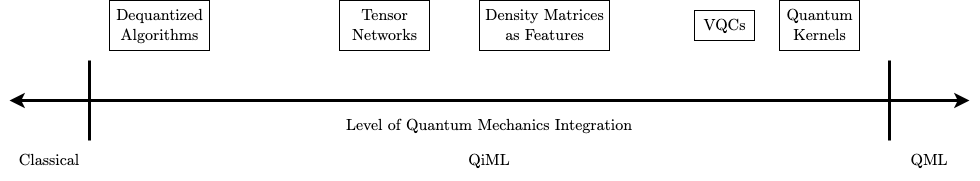
\includegraphics[width=\textwidth]{img/qiml_levels.png}
  \caption{A spectrum of machine learning approaches from classical to
    quantum-inspired to quantum-based
  methods~\cite{huynh2023quantuminspiredmachinelearningsurvey}.}
  \label{fig:qiml_levels}
\end{figure}

The primary difference between \gls{QML} and \gls{QiML} lies in their
reliance on quantum hardware. While \gls{QML} explores the use of
quantum computers to solve machine learning problems, \gls{QiML}
remains entirely within the classical computational realm, applying
quantum concepts without leveraging quantum hardware. This
distinction makes \gls{QiML} more accessible given current
technological limitations in quantum computing.

It is important to note that our research focuses on \gls{QML}, not
\gls{QiML}. In this project, we will directly employ simulated
quantum hardware and algorithms to explore how quantum computing can
enhance machine learning, specifically for sentiment analysis tasks
using transformer models.

\subsection{Quantum Neural Network}
\label{subsec:quantum_neural_network}
A \gls{QNN} is a machine learning architecture that
employs quantum computing principles. It has a set of trainable
parameters (\(\theta\)) that can be realised based on an initial
probability distribution. The goal of machine learning is to train
these parameters and achieve a probability distribution that closely
resembles the underlying problem. A model with high generalisation
ability can identify existing patterns in the testing data without
overfitting to the training data.

The specific approach involves providing the data to the quantum
model through a process called a data embedding strategy, which can
significantly impact the functional representation of the model. The
objective function is the expectation value of a variational
quantum circuit. These circuits make use of continuous variable group
rotations, allowing for the manipulation of quantum states.

Since there is no established framework for designing variational
quantum circuits, it is crucial to fine-tune the circuit
architecture, as it can directly affect the performance of the
quantum neural network model. Fortunately, many quantum computing
libraries, such as Pennylane and Qiskit, provide templates for
\glspl{VQC}.

\subsection{Data Embedding}
\label{subsec:data_embedding}
There are many encoding strategies for loading classical data into a
quantum computer but for this literature, we will only be discussing
about three encoding strategies. They are Angle embedding, Amplitude
embedding, Quantum Approximate Optimization Algorithm (QAOA)
embedding and Block Encoding.

\begin{itemize}
    % \setlength{\itemsep}{-1ex}
  \item Angle embedding~\cite{schuld2021supervised} is a
    straightforward strategy where classical data features are
    encoded into the angles of quantum gates. Each feature is mapped
    to the rotation angle of a qubit, typically using single-qubit
    rotation gates such as RX, RY, or RZ. To encode \(n\) features,
    Angle embedding requires \(n\) qubits, as each feature is
    directly assigned to a qubit's rotation. While this encoding
    method is straightforward, it can be resource-intensive for large
    datasets, as the number of qubits required grows rapidly with the
    number of features.

  \item Amplitude embedding~\cite{schuld2021supervised} is a more
    complex strategy that encodes classical data into the amplitudes
    of a quantum state. This method involves preparing a quantum
    state where the amplitudes of the state vector represent the
    classical data values. Given a classical data vector \( x = [x_1,
    x_2, \dots, x_n] \), the first step is to normalise the data. The
    normalisation is done by dividing each element by the Euclidean
    norm \( \|x\| \), where:

    \begin{equation}
      \| x \| = \sqrt{x_1^2 + x_2^2 + \dots + x_n^2}
    \end{equation}

    This ensures the total probability of the quantum state is 1. The
    normalised vector is:

    \begin{equation}
      \tilde{x} = \frac{1}{\| x \|} [x_1, x_2, \dots, x_n]
    \end{equation}

    Next, the normalised vector \( \tilde{x} \) is encoded into the
    amplitudes of a quantum state \( |\psi \rangle \), which can be
    represented as:

    \begin{equation}
      |\psi \rangle = \sum_{i=1}^{n} \tilde{x}_i |i\rangle
    \end{equation}

    where \( |i\rangle \) are the computational basis states. To
    encode \( n \) features, \( \log_2(n) \) qubits are required,
    assuming \( n \) is a power of two, because the quantum state
    must accommodate all \( n \) amplitudes, and \( \log_2(n) \)
    qubits are needed to create a state with \( n \) possible
    amplitudes. For example, if \( n = 4 \), the resulting quantum
    state would be:

    \begin{equation}
      |\psi \rangle = \tilde{x}_1 |00\rangle + \tilde{x}_2 |01\rangle
      + \tilde{x}_3 |10\rangle + \tilde{x}_4 |11\rangle
    \end{equation}

    This encoding strategy is particularly useful for applications
    that involve processing high-dimensional data, as it can
    significantly reduce the number of qubits required compared to
    other encoding methods.
  \item The Quantum Approximate Optimization Algorithm (QAOA)
    embedding~\cite{lloyd2020quantum} is a hybrid approach that
    encodes classical data into the parameters of a QAOA circuit.
    QAOA is originally designed for solving combinatorial
    optimisation problems but can be adapted for data encoding by
    associating the problem parameters with data features. The number
    of qubits required for QAOA embedding depends on the specific
    problem and the depth of the QAOA circuit but generally requires
    at least as many qubits as there are features to encode the data
    adequately. For \(n\) features, a minimum of \(n\) qubits is
    typically needed, with additional qubits possibly required
    depending on the circuit's complexity and the problem structure.
    In general, QAOA embedding requires several qubits that scale
    with the number of variables and constraints in the optimisation
    problem. This encoding strategy is particularly useful for
    solving combinatorial optimisation problems on quantum computers.
  \item Block encoding embeds a non-unitary operator as a sub-block
    of a larger unitary matrix,
    allowing non-unitary matrices to be processed within quantum circuits.
    In general, a matrix \( A \in \mathbb{C}^{N \times N} \), where
    \( N = 2^n \), can be block-encoded into a unitary matrix by
    extending the dimension of the matrix and adding ancilla qubits.

    The block-encoded matrix \( U \) can be represented as:
    \begin{equation}
      U =
      \begin{pmatrix}
        A & * \\
        * & *
      \end{pmatrix}
    \end{equation}

    The block-encoded form allows us to work with non-unitary
    operators in a quantum framework while maintaining the overall
    unitary evolution required by quantum mechanics.
    To perform block encoding, we use a combination of quantum
    oracles \( U_A \) and \( U_B \). The oracle \( U_A \) encodes the
    matrix elements \( A_{i,j} \) into the amplitude of an ancillary
    qubit, while \( U_B \) ensures proper indexing over the matrix
    entries. The combination of these operations allows the matrix \(
    A \) to be embedded as a block within a larger unitary matrix.
    This technique is particularly useful for quantum algorithms that
    involve manipulating large, structured, or sparse matrices, as it
    efficiently encodes the matrix into a quantum state without
    directly applying non-unitary operations. Block encoding is
    crucial for several quantum machine learning and linear algebra
    algorithms, enabling the practical implementation of otherwise
    challenging quantum computations.
\end{itemize}

\subsection{Variational Quantum Circuit}
\label{subsec:variational_quantum_circuit}
In classical neural networks, increasing the number of parameters
enhances the expressivity of the models. However, in quantum
circuits, having too many parameters can lead to redundancy because
over-parameterised circuits may not improve performance and can make
optimisation more challenging. Excess parameters can result in
entangled states that do not contribute meaningfully to the solution,
potentially causing the circuit to explore a larger, less relevant
portion of the parameter space. As mentioned earlier, there are no
standard frameworks for designing these architectures, resulting in
varying designs from one author to another. Nonetheless, quantum
computing libraries offer templates for \glspl{VQC} to facilitate their use.

\begin{equation}
  U(\theta) = \prod_{i=1}^{L} U_{i}(\theta_i)
\end{equation}

where \(L\) is the number of \gls{VQC}
iterations, \(U\) is the \gls{VQC} unitary,
\(\theta=(\theta_1,...,\theta_L )\) is a set of trainable parameters.

The \acrlong{VQC}~\cite{li2023quantum} consists of
repeated rotation gates applied to each qubit, along with CNOT gates
that entangle the qubits to form a highly entangled system. These
rotation gates, such as RX, RY, or RZ, adjust the qubit states based
on the trainable parameters. The CNOT gates, on the other hand,
create entanglement between pairs of qubits, enabling complex
interactions across the entire quantum system.

This combination of rotation and entangling gates allows the circuit
to explore a wide range of quantum states, enhancing its ability to
model complex functions and relationships within the data. By
fine-tuning the parameters of these gates, the quantum circuit can be
optimised to solve specific problems or recognise patterns in data.
However, designing these circuits requires careful consideration, as
the arrangement and number of gates can significantly impact the
circuit's performance and computational efficiency.

\subsection{Gradient Calculation}
\label{subsec:gradient_calculation}
The most common gradient calculation method in classical machine
learning is the back-propagation algorithm. This technique computes
the gradient of each function that the trainable parameters pass
through, using the chain rule to create an automatically
differentiable machine learning routine. In the context of quantum
machine learning, back-propagation can also be employed. However,
there’s a key difference: it requires access to the quantum state
vector. As a result, its application is limited to quantum simulators
rather than real quantum processing units (QPUs).

As a result, it is crucial to find alternative methods that can
operate on actual QPUs. One such alternative is the finite difference
method~\cite{Schuld_2019}, a form of numerical differentiation used
to approximate derivatives. The finite difference method estimates
the derivative of a function by evaluating the function at slightly
shifted parameter values and calculating the ratio of the change in
the function value to the change in the parameter.

However, while finite difference provides a useful approximation, it
can be quite unstable when used iteratively in processes such as
gradient descent. This instability arises because the method is
sensitive to numerical errors, which can accumulate over multiple
iterations, leading to inaccurate gradient estimates. Additionally,
near-term quantum hardware is inherently noisy, which further
exacerbates the inaccuracy of finite differences, making it
unreliable for precise optimisation tasks.

Another approach is the parameter shift rule~\cite{Schuld_2019},
which provides an exact derivative by evaluating the circuit twice
for each trainable parameter. Unlike finite difference methods, it
does not require a small perturbation but instead can use a
macroscopic shift. By optimising the shift to maximise the distance
in parameter space between the two circuit evaluations, the parameter
shift rule offers a robust and precise gradient estimation.

The parameter shift rule involves shifting the parameter by a fixed
amount in two directions and using the difference in the circuit's
outputs to calculate the gradient. Specifically, for a parameter
\(\theta\), the gradient  \(\pdv{f(\theta)}{\theta}\) is obtained by
evaluating the function \(f(\theta+s)\) and \(f(\theta-s)\) where
\(s\) is the shift value.

The exact derivative is then computed as:
\begin{equation}
\pdv{f(\theta)}{\theta}=\frac{f(\theta+s)-f(\theta-s))}{2sin(s)}
\end{equation}

This method is advantageous because it provides an unbiased estimator
of the gradient, ensuring convergence even when the gradient is
estimated with a single shot. In contrast, finite difference methods
approximate the derivative by evaluating the function at slightly
perturbed values of the parameter, which can be unstable and
sensitive to noise, especially in iterative processes like gradient
descent. Finite differences rely on a small perturbation to estimate
the gradient, which can accumulate numerical errors over multiple
iterations, leading to less accurate results.

However, the parameter shift rule does pose challenges. The number of
circuit evaluations required increases linearly with the number of
trainable parameters, which can limit the complexity of quantum
models. As the number of parameters grows, the computational
resources needed for gradient estimation also increase, potentially
making the process resource-intensive.

\subsection{Hybrid Classical-Quantum Autoencoder}
\label{subsec:hybrid_classical_quantum_autoencoder}
The \acrlong{VQC} uses angle embedding, where the input dimension is
restricted to a certain size due to the limitations of the available
qubits. This restriction limits the quantum circuit’s ability to
process larger input dimensions directly.

To address this limitation, a classical autoencoder is integrated into the
model, comprising an encoder and a decoder:

\begin{itemize}
\item The encoder acts as a compression mechanism, performing the
  squeezing of high-dimensional input data into a smaller latent
  space that fits the fixed input dimension of the quantum circuit.
  This is crucial for ensuring that the data can be processed within
  the qubit limitations of the \gls{VQC}.

\item The decoder performs the reverse operation, acting as an
  unsqueezing mechanism. After the quantum circuit processes the
  compressed data, the decoder expands the quantum-processed data
  back to its original size or another appropriate dimension for
  subsequent layers in the network.
\end{itemize}

By using this autoencoder structure, the model effectively bridges
the dimensional gap between high-dimensional classical data and the
qubit-limited quantum circuit. The encoder enables dimensionality
reduction while maintaining key features, and the decoder restores
the data to a useful size for further processing. This combination
allows the quantum circuit to be utilised efficiently within the
overall model without losing the ability to work with larger datasets.

\section{Quantum Transformers}
\label{sec:quantum_transformers}

\subsection{Basic Quantum Transformer}
\label{subsec:basic_quantum_transformer}
In 2021,~\citet{disipio2021dawn} proposed a Quantum Transformer that
replaces 5 linear layers with 5 Quantum layers which are ansatzes, 4
of which are in the multi-head attention, and 1 of which is in the
feed-forward network. The quantum layers use the basic entangler
layer template provided by PennyLane.

A variational quantum circuit cannot change the dimensionality of the
input but only rotate the state of the qubits, so the VQC is
sandwiched between 2 linear layers. A linear layer is used to
compress the dimension of the input to match the number of qubits and
another linear layer is used to uncompress the dimension of the
output to match the original dimension of the input so it can be
passed to the next layer.

This paper presents a conflicting scenario where the embedding
dimension and the number of qubits are mismatched. This incongruity
poses a significant challenge because the published code mandates
that the embedding dimension and the number of qubits align for the
multi-head attention mechanism to function correctly.

The parameters for training are as follows: 1 epoch, a batch size of
32, a vocabulary size of 50,000, a maximum sequence length of 64, an
embedding dimension of 8, 1 transformer block, 2 transformer heads
(the number of attention mechanisms in the multi-head attention
component), 1 quantum layer, and 2 qubits. The dataset used for
training and testing is the IMDB dataset, which consists of movie
reviews labelled as either positive or negative. Both the training
and testing sets contain 25,000 reviews each.

The author did not publish the results of the quantum transformer,
only mentioning that it took 100 hours to train the classifier for a
single epoch. I replicated the transformer and tested it on a subset
of the dataset, consisting of just 3,200 reviews. My results showed
that after 40 epochs, the training accuracy was 73\% and the testing
accuracy was 63\%. However, the model appeared to be overfitted, as
indicated by the train and test loss. More fine-tuning is needed to
increase the accuracy and prevent overfitting.

As this is one of the first papers on Quantum Transformers, I assume
that the author employed fundamental quantum machine learning
techniques to replace one or two components from classical to
quantum. By focusing on basic modifications, this entry-level code
provides a clear and accessible starting point for understanding the
process of converting Transformer components. This incremental
approach allows for a step-by-step conversion, making it easier to
grasp how quantum machine learning can be applied iteratively to
transition from classical to quantum models. This understanding is
crucial for developing more advanced quantum models in the future, as
it lays the groundwork for integrating quantum computing into
existing machine learning frameworks.

\subsection{Basic Quantum Vision Transformer}
\label{subsec:basic_quantum_vision_transformer}
In 2023,~\citet{Cara2024QVT} adapted~\citet{disipio2021dawn}’s basic
quantum transformer into a basic quantum vision
transformer.~\citet{Cara2024QVT} used 3 datasets, MNIST dataset,
Quark-Gluon dataset, and Electron-Photon dataset.

\begin{itemize}
  % \setlength{\itemsep}{-1ex}
\item MNIST dataset contains 70,000 1-channel 28x28 images of
  handwritten digits, which are labelled with the corresponding
  digit. The dataset is split into 60,000 images for training and
  10,000 images for testing.

\item Quark-Gluon consists of 933,206 3-channel 125x125 images, with
  half representing quarks and the other half gluons. Each of the
  three channels in the images corresponds to a specific component of
  the Compact Muon Solenoid (CMS) detector of the LHC: the inner
  tracking system (Tracks) that identifies charged particle tracks,
  the electromagnetic calorimeter (ECAL) that captures energy
  deposits from electromagnetic particles, and the hadronic
  calorimeter (HCAL) which detects energy deposits from hadrons.

\item Electron-Photon contains 498,000 2-channel 32x32 images, with
  half representing electrons and the other half representing
  photons. Here, only information from the CMS electromagnetic
  calorimeter (ECAL) is used. In particular, the first channel
  contains energy information (as in the Quark-Gluon dataset), and
  the second one contains timing information.
\end{itemize}

To convert the quantum transformer for text classification into a
quantum vision transformer for image classification, several
modifications are necessary. One major change involves splitting the
image into n patches and passing these patches through a linear layer
to flatten them before feeding them into the transformer. Another
significant change is appending the class tag to the very front of
the patches so that the multi-layer perceptron can use it for classification.

The parameters for training the quantum vision transformer are as
follows: 50 epochs, a patch size of 32, an embedding size of 8, 8
transformer blocks, 2 transformer heads, and 8 qubits. The training
results are as follows:

\begin{itemize}
  % \setlength{\itemsep}{-1ex}
\item For the MNIST dataset, the classical transformer achieved
  99.71\% accuracy, while the quantum transformer achieved 98.94\%.

\item For the Quark-Gluon dataset, the classical transformer achieved
  79.76\% accuracy, while the quantum transformer achieved 77.62\%.

\item For the Electron-Photon dataset, the classical transformer
  achieved 76.50\% accuracy, while the quantum transformer achieved 77.93\%.
\end{itemize}

From these results, we can see that the classical transformer
outperformed the quantum transformer on two of the datasets. For the
third dataset, the difference in performance between the classical
and quantum transformers is negligible.

\citet{Cara2024QVT} was aware that~\citet{disipio2021dawn}’s Quantum
Transformer requires a long training time, so they experimented with
different libraries to compare training durations. After testing
various options, they found that the library utilising tensor
networks was the fastest. This observation highlights that the choice
of quantum machine learning library can significantly influence not
only the training time but also the performance of the models.
Different libraries may offer optimisations, algorithms, and
implementations that impact efficiency and accuracy. Therefore,
selecting the appropriate library is crucial for achieving optimal
results in quantum machine learning experiments and applications.
This insight suggests that the performance of the Quantum Transformer
could be further improved by using tensor networks.

\subsection{Quantum Self Attention Neural Network}
\label{subsec:quantum_self_attention_neural_network}
In 2023,~\citet{li2023quantum} proposed a Quantum Self Attention
Neural Network for classification. This implementation has 2 parts.
The first part is in the quantum realm and the second part is in the
classical realm. The input is x, but this paper did not use any
positional encoding. The Quantum Self-Attention mechanisms are
connected sequentially and they are called the Quantum Self-Attention
Layer. Each layer has a set of four ansatzes. The outputs of the
final layer are averaged and fed into the second part which is a
classical fully connected layer for classification.

In the Quantum Self-Attention Layer, the embedding dimension of each
of the inputs has the same size as the number of qubits as each
element in the embedding is mapped to its corresponding qubits in the
ansatzes to encode the embeddings into their corresponding quantum
states. Then, a set of three ansatzes representing query, key, and
value is applied to each state. Note that it is the same set of
ansatzes applied to all the input states.

The measurement outputs of the query z-rotation part and the key
z-rotation part are computed through a Gaussian function to obtain
the quantum self-attention coefficients. We then calculate
classically weighted sums of the measurement outputs of the value and
add the inputs to get the outputs of the current layer where the
weights are the normalised coefficient.

All the ansatz parameters and weight are initialised from a Gaussian
distribution with zero mean and 0.01 standard deviation, and the bias
is initialised to zero. Here, the ansatz parameters are not
initialised uniformly from \([0, 2\pi)\) is mainly due to the
residual scheme applied before the output of the current layer. They
are using the parameter shift rule for the gradient calculation.

The QSANN is not a transformer as it lacks two key components:
multi-head attention and position encoding. In their study, two
simple synthetic datasets were used, named MC and RP. The MC dataset
contains 17 words and 130 sentences (70 for training, 30 for
development, and 30 for testing), with each sentence consisting of 3
or 4 words. The RP dataset contains 115 words and 105 sentences (74
for training and 31 for testing), with each sentence containing 4 words.

The results are somewhat unusual. The model achieved 100\% accuracy
on both training and testing for the MC dataset. For the RP dataset,
the training accuracy was 95.35\% and the testing accuracy was
67.74\%. The second dataset's results seem more reasonable than the
first. The anomalous result for the MC dataset might be due to the
extremely small size of the dataset, which contains only 17 unique words.

Unlike previous authors, these authors provide a comprehensive and
detailed explanation of their implementation, starting from the
basics of quantum computing and progressing through to the classical
gradient chain rule and the quantum parameter shift rule. They also
include clear and informative diagrams to aid in their explanations.
This thorough approach ensures that readers can follow the concepts
and methodologies step by step. The depth of detail and clarity in
this paper have been incredibly helpful in enhancing my understanding
of how Quantum Transformers are implemented on quantum computers.
Their meticulous explanation and visual aids make complex concepts
more accessible and comprehensible, bridging the gap between
classical and quantum machine learning techniques. This paper stands
out as a valuable resource for anyone looking to grasp the
intricacies of Quantum Transformers.

\subsection{Quantum Vision Transformer}
\label{subsec:quantum_vision_transformer}
In 2024,~\citet{Cherrat_2024} proposed two Quantum Vision
Transformers. They designed a custom data loader with two registers.
The top register loads the norms of each row of the input patch
vector, while the lower register sequentially loads each row by
applying the vector loader and its adjoint for each row, using CNOTs
controlled by the corresponding qubit of the top register. In
essence, they use amplitude encoding to transfer classical data into
the quantum realm.

\citet{Cherrat_2024} also designed three circuits which they called
the orthogonal layer: Pyramid, X, and Butterfly. Instead of using
CNOTs to entangle the qubits, they employed a different entangling
gate known as the RBS gate. The process begins with a Hadamard gate
applied to each of the two qubits, followed by a two-qubit CZ gate.
This is then followed by a Ry rotation gate on each qubit, where the
top qubit is rotated by \(\frac{\theta}{2}\) and the bottom qubit by
\(-\frac{\theta}{2}\). Another two-qubit CZ gate is applied, and
finally, a Hadamard gate is applied to each qubit.

The first transformer they proposed is called the Quantum Orthogonal
Transformer. This circuit begins by loading the input patch vector,
followed by a trainable quantum orthogonal layer. Next, an inverse
data loader for the input patch vector creates a state where the
probability of measuring 1 on the first qubit is exactly the square
of the attention coefficient. Another circuit, the Orthogonal
Patch-wise Neural Network, is similar but lacks the inverse data
loader. Its output, the feature vector, combined with the attention
coefficient, can then be classically processed to obtain the attention vectors.

Additionally, they designed a circuit called Direct Quantum Attention
to calculate the attention output within the quantum computer. This
circuit consists of two registers: the top register loads the
attention coefficients, while the bottom register contains a data
loader for the input patch vector. The loader is controlled by the
top register using a CNOT gate, so the input patch vector is loaded
with all rows rescaled according to the attention coefficients. The
data is then passed through a quantum orthogonal layer, which
performs matrix multiplication between the feature vector and the
newly encoded vector. The output of the second register is the
attention vector. With this tool, the Quantum Orthogonal Transformer
with Direct Quantum Attention can perform attention calculations
entirely within the quantum realm.

They also proposed another Quantum Vision Transformer implementation,
claiming it utilises quantum-native linear algebraic operations that
cannot be efficiently performed classically. However, they did not
publish their code, and Cara's attempts to replicate their work were
unsuccessful, noting that some explanations in their work were
unclear. Therefore, this implementation will only be briefly mentioned.

They trained and tested their models on the MedMNIST dataset, a
collection of 12 pre-processed, two-dimensional, open-source medical
image datasets. Their results demonstrated that the orthogonal
transformer and the compound transformer, both of which implement
non-trivial quantum attention mechanisms, delivered very competitive
performances compared to the classical vision transformer. Notably,
these quantum transformers outperformed the classical vision
transformer on 7 out of the 12 MedMNIST datasets.

The authors tested their models on actual quantum computers,
providing a practical demonstration of their implementation.
Furthermore, they developed a Quantum Transformer capable of
calculating the attention output directly on the quantum computer.
This approach contrasts with previous quantum transformers, which
rely on classical computation for attention calculation. By
integrating the attention mechanism fully within the quantum
framework, their Quantum Transformer potentially offers improved
performance and efficiency, showcasing a significant advancement in
the application of quantum computing to machine learning tasks. This
novel approach demonstrates the feasibility and benefits of
performing more complex computations directly on quantum hardware.

\section{Synthesis}
\label{sec:synthesis}
All the mentioned models use variational quantum circuits to
replace classical neural networks with quantum neural networks. Most
of these models calculate the attention output classically,
maintaining some dependence on classical computation. The only model
that calculates the attention output directly on the quantum computer
is the direct quantum attention add-on for ~\citet{Cherrat_2024}’s
model, setting it apart as a more integrated quantum solution.

Despite these differences, a common feature among all models is the
use of a classical fully connected layer for classification. This
reliance on classical components means that all these models are
hybrid quantum transformers rather than purely quantum-native
transformers. The hybrid approach leverages the strengths of both
quantum and classical computing but also indicates that fully
quantum-native transformers are still under development.

Moreover, while these models share the goal of enhancing
computational efficiency and performance through quantum computing,
their varying approaches highlight the experimental nature of the
field. For instance, the choice of entangling gates, data encoding
strategies, and specific quantum operations differ across models,
reflecting ongoing exploration of optimal techniques.

Interestingly, none of the papers discuss the issue of barren
plateaus, a problem in quantum neural networks where gradients vanish
during training. This phenomenon can severely affect training
efficiency or even bring it to a halt, as the gradient of the model
tends to zero in all directions. According to~\citet{McClean_2018},
quantum neural networks must be shallow and use a limited number of
qubits to remain trainable, which contradicts the vision of
high-dimensional, million-qubit quantum machine learning models. This
issue underscores a significant challenge in the field that future
research must address to realise the full potential of quantum neural networks.
